% Options for packages loaded elsewhere
\PassOptionsToPackage{unicode}{hyperref}
\PassOptionsToPackage{hyphens}{url}
%
\documentclass[
  12pt,
  norsk,
]{article}
\usepackage{amsmath,amssymb}
\usepackage{lmodern}
\usepackage{setspace}
\usepackage{ifxetex,ifluatex}
\ifnum 0\ifxetex 1\fi\ifluatex 1\fi=0 % if pdftex
  \usepackage[T1]{fontenc}
  \usepackage[utf8]{inputenc}
  \usepackage{textcomp} % provide euro and other symbols
\else % if luatex or xetex
  \usepackage{unicode-math}
  \defaultfontfeatures{Scale=MatchLowercase}
  \defaultfontfeatures[\rmfamily]{Ligatures=TeX,Scale=1}
\fi
% Use upquote if available, for straight quotes in verbatim environments
\IfFileExists{upquote.sty}{\usepackage{upquote}}{}
\IfFileExists{microtype.sty}{% use microtype if available
  \usepackage[]{microtype}
  \UseMicrotypeSet[protrusion]{basicmath} % disable protrusion for tt fonts
}{}
\makeatletter
\@ifundefined{KOMAClassName}{% if non-KOMA class
  \IfFileExists{parskip.sty}{%
    \usepackage{parskip}
  }{% else
    \setlength{\parindent}{0pt}
    \setlength{\parskip}{6pt plus 2pt minus 1pt}}
}{% if KOMA class
  \KOMAoptions{parskip=half}}
\makeatother
\usepackage{xcolor}
\IfFileExists{xurl.sty}{\usepackage{xurl}}{} % add URL line breaks if available
\IfFileExists{bookmark.sty}{\usepackage{bookmark}}{\usepackage{hyperref}}
\hypersetup{
  pdftitle={Innlevering 2},
  pdfauthor={Innlevering 2 i Data Science 2021 - Maren Sognefest og Daniel Karstad},
  pdflang={no-NB},
  hidelinks,
  pdfcreator={LaTeX via pandoc}}
\urlstyle{same} % disable monospaced font for URLs
\usepackage[margin=1in]{geometry}
\usepackage{color}
\usepackage{fancyvrb}
\newcommand{\VerbBar}{|}
\newcommand{\VERB}{\Verb[commandchars=\\\{\}]}
\DefineVerbatimEnvironment{Highlighting}{Verbatim}{commandchars=\\\{\}}
% Add ',fontsize=\small' for more characters per line
\usepackage{framed}
\definecolor{shadecolor}{RGB}{248,248,248}
\newenvironment{Shaded}{\begin{snugshade}}{\end{snugshade}}
\newcommand{\AlertTok}[1]{\textcolor[rgb]{0.94,0.16,0.16}{#1}}
\newcommand{\AnnotationTok}[1]{\textcolor[rgb]{0.56,0.35,0.01}{\textbf{\textit{#1}}}}
\newcommand{\AttributeTok}[1]{\textcolor[rgb]{0.77,0.63,0.00}{#1}}
\newcommand{\BaseNTok}[1]{\textcolor[rgb]{0.00,0.00,0.81}{#1}}
\newcommand{\BuiltInTok}[1]{#1}
\newcommand{\CharTok}[1]{\textcolor[rgb]{0.31,0.60,0.02}{#1}}
\newcommand{\CommentTok}[1]{\textcolor[rgb]{0.56,0.35,0.01}{\textit{#1}}}
\newcommand{\CommentVarTok}[1]{\textcolor[rgb]{0.56,0.35,0.01}{\textbf{\textit{#1}}}}
\newcommand{\ConstantTok}[1]{\textcolor[rgb]{0.00,0.00,0.00}{#1}}
\newcommand{\ControlFlowTok}[1]{\textcolor[rgb]{0.13,0.29,0.53}{\textbf{#1}}}
\newcommand{\DataTypeTok}[1]{\textcolor[rgb]{0.13,0.29,0.53}{#1}}
\newcommand{\DecValTok}[1]{\textcolor[rgb]{0.00,0.00,0.81}{#1}}
\newcommand{\DocumentationTok}[1]{\textcolor[rgb]{0.56,0.35,0.01}{\textbf{\textit{#1}}}}
\newcommand{\ErrorTok}[1]{\textcolor[rgb]{0.64,0.00,0.00}{\textbf{#1}}}
\newcommand{\ExtensionTok}[1]{#1}
\newcommand{\FloatTok}[1]{\textcolor[rgb]{0.00,0.00,0.81}{#1}}
\newcommand{\FunctionTok}[1]{\textcolor[rgb]{0.00,0.00,0.00}{#1}}
\newcommand{\ImportTok}[1]{#1}
\newcommand{\InformationTok}[1]{\textcolor[rgb]{0.56,0.35,0.01}{\textbf{\textit{#1}}}}
\newcommand{\KeywordTok}[1]{\textcolor[rgb]{0.13,0.29,0.53}{\textbf{#1}}}
\newcommand{\NormalTok}[1]{#1}
\newcommand{\OperatorTok}[1]{\textcolor[rgb]{0.81,0.36,0.00}{\textbf{#1}}}
\newcommand{\OtherTok}[1]{\textcolor[rgb]{0.56,0.35,0.01}{#1}}
\newcommand{\PreprocessorTok}[1]{\textcolor[rgb]{0.56,0.35,0.01}{\textit{#1}}}
\newcommand{\RegionMarkerTok}[1]{#1}
\newcommand{\SpecialCharTok}[1]{\textcolor[rgb]{0.00,0.00,0.00}{#1}}
\newcommand{\SpecialStringTok}[1]{\textcolor[rgb]{0.31,0.60,0.02}{#1}}
\newcommand{\StringTok}[1]{\textcolor[rgb]{0.31,0.60,0.02}{#1}}
\newcommand{\VariableTok}[1]{\textcolor[rgb]{0.00,0.00,0.00}{#1}}
\newcommand{\VerbatimStringTok}[1]{\textcolor[rgb]{0.31,0.60,0.02}{#1}}
\newcommand{\WarningTok}[1]{\textcolor[rgb]{0.56,0.35,0.01}{\textbf{\textit{#1}}}}
\usepackage{longtable,booktabs,array}
\usepackage{calc} % for calculating minipage widths
% Correct order of tables after \paragraph or \subparagraph
\usepackage{etoolbox}
\makeatletter
\patchcmd\longtable{\par}{\if@noskipsec\mbox{}\fi\par}{}{}
\makeatother
% Allow footnotes in longtable head/foot
\IfFileExists{footnotehyper.sty}{\usepackage{footnotehyper}}{\usepackage{footnote}}
\makesavenoteenv{longtable}
\usepackage{graphicx}
\makeatletter
\def\maxwidth{\ifdim\Gin@nat@width>\linewidth\linewidth\else\Gin@nat@width\fi}
\def\maxheight{\ifdim\Gin@nat@height>\textheight\textheight\else\Gin@nat@height\fi}
\makeatother
% Scale images if necessary, so that they will not overflow the page
% margins by default, and it is still possible to overwrite the defaults
% using explicit options in \includegraphics[width, height, ...]{}
\setkeys{Gin}{width=\maxwidth,height=\maxheight,keepaspectratio}
% Set default figure placement to htbp
\makeatletter
\def\fps@figure{htbp}
\makeatother
\setlength{\emergencystretch}{3em} % prevent overfull lines
\providecommand{\tightlist}{%
  \setlength{\itemsep}{0pt}\setlength{\parskip}{0pt}}
\setcounter{secnumdepth}{-\maxdimen} % remove section numbering
\ifxetex
  % Load polyglossia as late as possible: uses bidi with RTL langages (e.g. Hebrew, Arabic)
  \usepackage{polyglossia}
  \setmainlanguage[]{norsk}
\else
  \usepackage[main=norsk]{babel}
% get rid of language-specific shorthands (see #6817):
\let\LanguageShortHands\languageshorthands
\def\languageshorthands#1{}
\fi
\ifluatex
  \usepackage{selnolig}  % disable illegal ligatures
\fi

\title{Innlevering 2}
\author{Innlevering 2 i Data Science 2021 - Maren Sognefest og Daniel
Karstad}
\date{}

\begin{document}
\maketitle

\setstretch{1.5}
\begin{Shaded}
\begin{Highlighting}[]
\NormalTok{echo }\OtherTok{=} \ConstantTok{FALSE} 
\FunctionTok{library}\NormalTok{(modelr) }
\FunctionTok{library}\NormalTok{(ggplot2) }
\FunctionTok{library}\NormalTok{(knitr) }
\FunctionTok{library}\NormalTok{(tinytex) }
\FunctionTok{library}\NormalTok{(tidyverse) }
\end{Highlighting}
\end{Shaded}

\begin{verbatim}
## -- Attaching packages --------------------------------------- tidyverse 1.3.1 --
\end{verbatim}

\begin{verbatim}
## v tibble  3.1.3     v dplyr   1.0.7
## v tidyr   1.1.3     v stringr 1.4.0
## v readr   2.0.0     v forcats 0.5.1
## v purrr   0.3.4
\end{verbatim}

\begin{verbatim}
## -- Conflicts ------------------------------------------ tidyverse_conflicts() --
## x dplyr::filter() masks stats::filter()
## x dplyr::lag()    masks stats::lag()
\end{verbatim}

\begin{Shaded}
\begin{Highlighting}[]
\FunctionTok{library}\NormalTok{(ggpubr)}
\FunctionTok{data}\NormalTok{(}\StringTok{\textquotesingle{}heights\textquotesingle{}}\NormalTok{, }\AttributeTok{package =} \StringTok{\textquotesingle{}modelr\textquotesingle{}}\NormalTok{)}
\NormalTok{hoyde}\OtherTok{\textless{}{-}}\FunctionTok{data.frame}\NormalTok{(heights) }\CommentTok{\#kopi av datasettet "heights", kalt "hoyde"}
\FunctionTok{tracemem}\NormalTok{(hoyde)}\SpecialCharTok{==}\FunctionTok{tracemem}\NormalTok{(heights)}
\end{Highlighting}
\end{Shaded}

\begin{verbatim}
## [1] FALSE
\end{verbatim}

\hypertarget{er-det-huxf8yde-som-bestemmer-inntekt}{%
\section{Er det høyde som bestemmer
inntekt?}\label{er-det-huxf8yde-som-bestemmer-inntekt}}

Denne artikkelen skal ta for seg om det er en, og eventuelt hvilken,
sammenheng det er mellom høyde og inntekt. Ved hjelp av flere analyser,
skal vi bruke datasettet \textbf{heights} fra pakken \textbf{modelr}
skal vi prøve å finne ut om det er en sammenheng. Kan det stemme at høye
personer tjener mest?

I analyse-delen av artikkelen vil vi bruke ulike \textbf{plots} for å
analysere spørsmålet, og komme frem til en konklusjon.

\begin{itemize}
\item
  ca 1 side litteraturgjennomgang
\item
  Start analyse med å lage din egen versjon av datasettet. Kall det for
  hoyde og jobb med dette.
\end{itemize}

\begin{Shaded}
\begin{Highlighting}[]
\NormalTok{knitr}\SpecialCharTok{::}\FunctionTok{kable}\NormalTok{(}\FunctionTok{summary}\NormalTok{(heights[}\DecValTok{1}\SpecialCharTok{:}\DecValTok{8}\NormalTok{]), }\StringTok{"pipe"}\NormalTok{)}
\end{Highlighting}
\end{Shaded}

\begin{longtable}[]{@{}
  >{\raggedright\arraybackslash}p{(\columnwidth - 16\tabcolsep) * \real{0.03}}
  >{\raggedright\arraybackslash}p{(\columnwidth - 16\tabcolsep) * \real{0.15}}
  >{\raggedright\arraybackslash}p{(\columnwidth - 16\tabcolsep) * \real{0.11}}
  >{\raggedright\arraybackslash}p{(\columnwidth - 16\tabcolsep) * \real{0.12}}
  >{\raggedright\arraybackslash}p{(\columnwidth - 16\tabcolsep) * \real{0.12}}
  >{\raggedright\arraybackslash}p{(\columnwidth - 16\tabcolsep) * \real{0.13}}
  >{\raggedright\arraybackslash}p{(\columnwidth - 16\tabcolsep) * \real{0.10}}
  >{\raggedright\arraybackslash}p{(\columnwidth - 16\tabcolsep) * \real{0.12}}
  >{\raggedright\arraybackslash}p{(\columnwidth - 16\tabcolsep) * \real{0.13}}@{}}
\toprule
& income & height & weight & age & marital & sex & education & afqt \\
\midrule
\endhead
& Min. : 0.0 & Min. :52.0 & Min. : 76.0 & Min. :47.00 & single :1124 &
male :3402 & Min. : 1.00 & Min. : 0.00 \\
& 1st Qu.: 165.5 & 1st Qu.:64.0 & 1st Qu.:157.0 & 1st Qu.:49.00 &
married :3806 & female:3604 & 1st Qu.:12.00 & 1st Qu.: 15.12 \\
& Median : 29589.5 & Median :67.0 & Median :184.0 & Median :51.00 &
separated: 366 & NA & Median :12.00 & Median : 36.76 \\
& Mean : 41203.9 & Mean :67.1 & Mean :188.3 & Mean :51.33 & divorced
:1549 & NA & Mean :13.22 & Mean : 41.21 \\
& 3rd Qu.: 55000.0 & 3rd Qu.:70.0 & 3rd Qu.:212.0 & 3rd Qu.:53.00 &
widowed : 161 & NA & 3rd Qu.:15.00 & 3rd Qu.: 65.24 \\
& Max. :343830.0 & Max. :84.0 & Max. :524.0 & Max. :56.00 & NA & NA &
Max. :20.00 & Max. :100.00 \\
& NA & NA & NA's :95 & NA & NA & NA & NA's :10 & NA's :262 \\
\bottomrule
\end{longtable}

\begin{itemize}
\tightlist
\item
  Beskrivende statistikk, dvs. kort beskrivelse av dataen
\end{itemize}

Her er sammendraget over statistikken vår. Man har kolonner med inntekt
i dollar, høyde i inches, vekt i pounds, alder, sivilstatus, kjønn,
utdannelse og score på Armed Forces Qualitication Test. Under er
sammendraget av vårt modifiserte datasett. Her har vi gjort dataen til
europeiske standarderer; vi bruker høyde i cm og vekt i kg, i tillegg
til at inntekten er i norske kroner. Vi har også lagt til bmi.

\begin{Shaded}
\begin{Highlighting}[]
\NormalTok{hoyde}\SpecialCharTok{$}\NormalTok{hoyde\_cm }\OtherTok{\textless{}{-}}\NormalTok{ hoyde}\SpecialCharTok{$}\NormalTok{height}\SpecialCharTok{*}\FloatTok{2.54}
\end{Highlighting}
\end{Shaded}

\begin{verbatim}
## tracemem[0x00000000276205a8 -> 0x0000000024d445f0]: eval eval withVisible withCallingHandlers handle timing_fn evaluate_call <Anonymous> evaluate in_dir eng_r block_exec call_block process_group.block process_group withCallingHandlers process_file <Anonymous> <Anonymous> 
## tracemem[0x0000000024d445f0 -> 0x0000000024d44430]: $<-.data.frame $<- eval eval withVisible withCallingHandlers handle timing_fn evaluate_call <Anonymous> evaluate in_dir eng_r block_exec call_block process_group.block process_group withCallingHandlers process_file <Anonymous> <Anonymous>
\end{verbatim}

\begin{Shaded}
\begin{Highlighting}[]
\NormalTok{hoyde}\SpecialCharTok{$}\NormalTok{inntekt\_nok }\OtherTok{\textless{}{-}}\NormalTok{ hoyde}\SpecialCharTok{$}\NormalTok{income}\SpecialCharTok{*}\FloatTok{8.5}
\NormalTok{hoyde}\SpecialCharTok{$}\NormalTok{vekt\_kg }\OtherTok{\textless{}{-}}\NormalTok{ hoyde}\SpecialCharTok{$}\NormalTok{weight}\SpecialCharTok{/}\FloatTok{2.2}
\NormalTok{hoyde}\SpecialCharTok{$}\NormalTok{bmi }\OtherTok{\textless{}{-}}\NormalTok{ hoyde}\SpecialCharTok{$}\NormalTok{vekt\_kg}\SpecialCharTok{/}\NormalTok{(hoyde}\SpecialCharTok{$}\NormalTok{hoyde\_cm}\SpecialCharTok{/}\DecValTok{100}\NormalTok{)}\SpecialCharTok{/}\NormalTok{(hoyde}\SpecialCharTok{$}\NormalTok{hoyde\_cm}\SpecialCharTok{/}\DecValTok{100}\NormalTok{)}
\end{Highlighting}
\end{Shaded}

\begin{Shaded}
\begin{Highlighting}[]
\NormalTok{hoyde}\SpecialCharTok{$}\NormalTok{height\_cmInt }\OtherTok{\textless{}{-}} \ConstantTok{NULL}
\NormalTok{hoyde}\SpecialCharTok{$}\NormalTok{weight }\OtherTok{\textless{}{-}} \ConstantTok{NULL}
\NormalTok{hoyde}\SpecialCharTok{$}\NormalTok{height }\OtherTok{\textless{}{-}} \ConstantTok{NULL}
\NormalTok{hoyde}\SpecialCharTok{$}\NormalTok{income }\OtherTok{\textless{}{-}} \ConstantTok{NULL}

\NormalTok{knitr}\SpecialCharTok{::}\FunctionTok{kable}\NormalTok{(}\FunctionTok{summary}\NormalTok{(hoyde[}\DecValTok{1}\SpecialCharTok{:}\DecValTok{9}\NormalTok{]), }\StringTok{"pipe"}\NormalTok{)}
\end{Highlighting}
\end{Shaded}

\begin{longtable}[]{@{}
  >{\raggedright\arraybackslash}p{(\columnwidth - 18\tabcolsep) * \real{0.02}}
  >{\raggedright\arraybackslash}p{(\columnwidth - 18\tabcolsep) * \real{0.11}}
  >{\raggedright\arraybackslash}p{(\columnwidth - 18\tabcolsep) * \real{0.11}}
  >{\raggedright\arraybackslash}p{(\columnwidth - 18\tabcolsep) * \real{0.09}}
  >{\raggedright\arraybackslash}p{(\columnwidth - 18\tabcolsep) * \real{0.11}}
  >{\raggedright\arraybackslash}p{(\columnwidth - 18\tabcolsep) * \real{0.11}}
  >{\raggedright\arraybackslash}p{(\columnwidth - 18\tabcolsep) * \real{0.11}}
  >{\raggedright\arraybackslash}p{(\columnwidth - 18\tabcolsep) * \real{0.12}}
  >{\raggedright\arraybackslash}p{(\columnwidth - 18\tabcolsep) * \real{0.11}}
  >{\raggedright\arraybackslash}p{(\columnwidth - 18\tabcolsep) * \real{0.11}}@{}}
\toprule
& age & marital & sex & education & afqt & hoyde\_cm & inntekt\_nok &
vekt\_kg & bmi \\
\midrule
\endhead
& Min. :47.00 & single :1124 & male :3402 & Min. : 1.00 & Min. : 0.00 &
Min. :132.1 & Min. : 0 & Min. : 34.55 & Min. :12.90 \\
& 1st Qu.:49.00 & married :3806 & female:3604 & 1st Qu.:12.00 & 1st Qu.:
15.12 & 1st Qu.:162.6 & 1st Qu.: 1407 & 1st Qu.: 71.36 & 1st
Qu.:25.14 \\
& Median :51.00 & separated: 366 & NA & Median :12.00 & Median : 36.76 &
Median :170.2 & Median : 251511 & Median : 83.64 & Median :28.38 \\
& Mean :51.33 & divorced :1549 & NA & Mean :13.22 & Mean : 41.21 & Mean
:170.4 & Mean : 350234 & Mean : 85.59 & Mean :29.37 \\
& 3rd Qu.:53.00 & widowed : 161 & NA & 3rd Qu.:15.00 & 3rd Qu.: 65.24 &
3rd Qu.:177.8 & 3rd Qu.: 467500 & 3rd Qu.: 96.36 & 3rd Qu.:32.35 \\
& Max. :56.00 & NA & NA & Max. :20.00 & Max. :100.00 & Max. :213.4 &
Max. :2922555 & Max. :238.18 & Max. :75.15 \\
& NA & NA & NA & NA's :10 & NA's :262 & NA & NA & NA's :95 & NA's :95 \\
\bottomrule
\end{longtable}

\hypertarget{eda-vha.-ggplot-av-datasettet.}{%
\section{EDA (vha. ggplot) av
datasettet.}\label{eda-vha.-ggplot-av-datasettet.}}

\begin{Shaded}
\begin{Highlighting}[]
\FunctionTok{library}\NormalTok{(ggplot2) }\CommentTok{\#data visualization}
\FunctionTok{library}\NormalTok{(dplyr) }\CommentTok{\#data manipulation}
\FunctionTok{library}\NormalTok{(ISLR) }\CommentTok{\#for the dataset}

\FunctionTok{ggplot}\NormalTok{(}\AttributeTok{data =}\NormalTok{ hoyde, }\FunctionTok{aes}\NormalTok{(}\AttributeTok{x =}\NormalTok{ inntekt\_nok, }\AttributeTok{y =}\NormalTok{ hoyde\_cm)) }\SpecialCharTok{+} \FunctionTok{geom\_point}\NormalTok{()}
\end{Highlighting}
\end{Shaded}

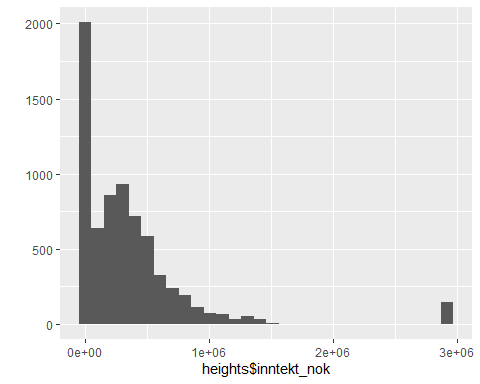
\includegraphics{Innlevering-2_files/figure-latex/unnamed-chunk-5-1.pdf}

\begin{Shaded}
\begin{Highlighting}[]
\FunctionTok{qplot}\NormalTok{(hoyde}\SpecialCharTok{$}\NormalTok{inntekt\_nok, }\AttributeTok{geom=}\StringTok{"histogram"}\NormalTok{) }
\end{Highlighting}
\end{Shaded}

\begin{verbatim}
## `stat_bin()` using `bins = 30`. Pick better value with `binwidth`.
\end{verbatim}

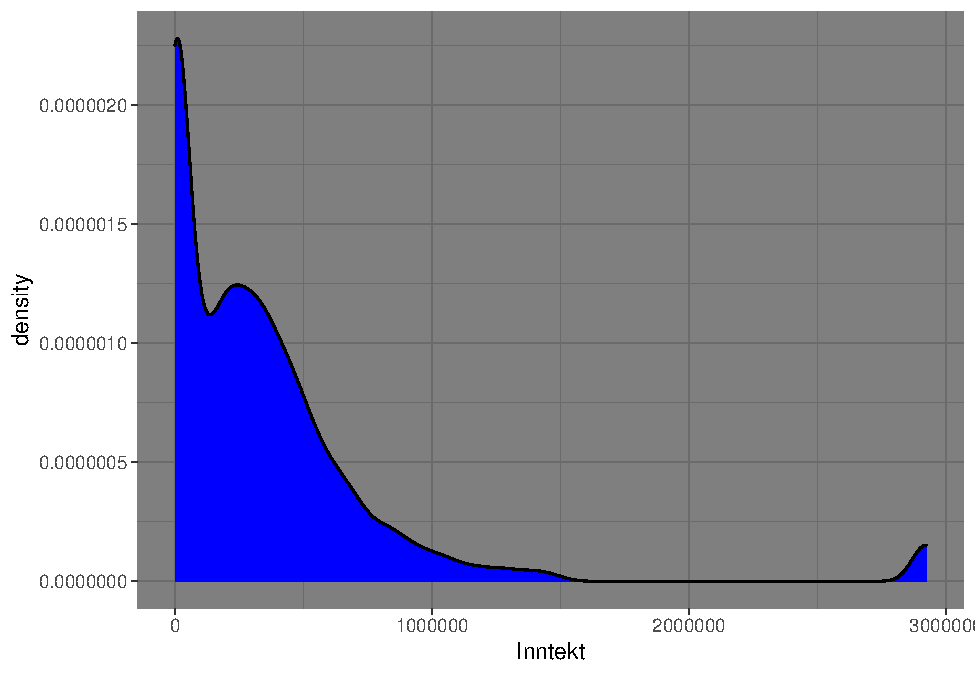
\includegraphics{Innlevering-2_files/figure-latex/unnamed-chunk-6-1.pdf}

Utliggerne til høyre er der fordi det er beregnet gjennomsnittsinntekt
av de to prosentene med høyest inntekt. Dette gjennomsnittet er brukt,
og har erstattet alle de øverste verdiene.

Som man kan se utfra histogrammet er det med flere uten inntekt i
datasettet. Det kan man også se slik:

\begin{Shaded}
\begin{Highlighting}[]
\FunctionTok{sum}\NormalTok{(hoyde}\SpecialCharTok{$}\NormalTok{inntekt\_nok }\SpecialCharTok{==} \DecValTok{0}\NormalTok{)}
\end{Highlighting}
\end{Shaded}

\begin{verbatim}
## [1] 1740
\end{verbatim}

Det er altå 1740 personer uten inntekt med i datasettet.

\begin{itemize}
\tightlist
\item
  Regresjonsanalyse (dokumentetLiten introduksjon til å kjøre
  regresjonsanalyser i Rkan være til hjelp)
\end{itemize}

\begin{Shaded}
\begin{Highlighting}[]
\NormalTok{x }\OtherTok{\textless{}{-}}\NormalTok{ hoyde}\SpecialCharTok{$}\NormalTok{hoyde\_cm}
\NormalTok{y }\OtherTok{\textless{}{-}}\NormalTok{ hoyde}\SpecialCharTok{$}\NormalTok{inntekt\_nok}
\end{Highlighting}
\end{Shaded}

-- Vi benytter hele datasettet, men vil kjøre endelig modell også mot
reduserte datasett (uten 2\% topp inntekt og uten inntekt 0) for å teste
modellens robusthet (huskfilterfunksjonen fraTidyverse)--L ag to nye
variabler height\_cm og weight\_kg ( vha. mutate()) der du konverterer
variableneheight (inch) og weight (pound) til metrisk standard.

-- Lag også en ny variabel bmi (der bmi=vekt i kg/(høyde i cm)ˆ2).--Lag
en forenklet utgave av variabelen marital, dvs. married not-married. Kan
enkelt gjøres vha.

Totalt skal minst 6 modeller estimeres

\begin{itemize}
\item
  Resultatet fra estimeringen skal rapporteres vha. huxreg(). Se
  dokumentet ex\_reg\_tables.pdf underFiler \textgreater{} Assignment 2
  på Canvas, hvis du har glemt hvordan det gjøres. Tips: angir du en
  liste somførste argument til huxreg() kan du styre hva modellene skal
  hete, f.eks (gir også t-verdier istedenforstandard error)
\item
  Den endelige modellen skal testes for robusthet på et datasett uten de
  2\% høyeste inntektene og på etdatasett som i tillegg ikke inneholder
  observasjoner der inntekten er 0.
\item
  Disse modellene på redusert datasett teller med blant de 6.Minst en av
  modellene skal inneholde interaksjon mht. variabelen sex. (Se eksempel
  7.10 i dokumentetLiten
  intro){]}(\url{https://elastic-turing-41462a.netlify.app/presentations_ag/intro_econometrics/w_4c1_and_4c3})))
\item
  Det skal gjøres test av koeffisientene vha. linearHypothesis() fra car
  pakken
\item
  Residualene fra endelig modell skal legges til datasettet hoyde.
  height\_cm skal plottes mot residualenefor `facet\_grid(sex
  \textasciitilde{} factor(married, labels = c(``not married,''
  ``married'')))'
\item
  Plot av samtlige observasjoner svakt i bakgrunnen kan en få til med
\item
  Konklusjon Svar på spørsmålet: Er det høyde som bestemmer inntekt?
\end{itemize}

\hypertarget{referanser}{%
\section{Referanser}\label{referanser}}

::: \{\#refs\} :::

\end{document}
